\documentclass[a4paper,11pt]{report}

\usepackage[frenchb]{babel}
\usepackage[utf8]{inputenc}
\usepackage{wrapfig}
\usepackage{graphicx}
\usepackage {amsmath}
\usepackage{amssymb}
\usepackage{amsthm}
\usepackage{mathrsfs}
\usepackage{soul}
\usepackage{algorithm,algorithmic}
\usepackage{listings}
\usepackage{array}
\usepackage[toc,page]{appendix} 
\usepackage[top=2.5cm, bottom=3cm, left=3cm, right=3cm]{geometry}


\begin{document}

%%%%%%%%%%%%%%%%%%%%%%%%%%%%%%%%%%%%%%%%%%%%%%%%%%%
%page de garde
\begin{figure}
   
\includegraphics[scale = 0.75]{HeaderPagedeGarde.PNG}
\end{figure}


\author{Maxime Escourbiac \\ Responsable ISIMA : Marie AGIER}
\title{
   Rapport préliminaire \\ Gestion des projets ISIMA \\
  \bigskip
   \large{
     Business Intelligence
   }
}
\date{9 Mai 2012}
\maketitle

\newpage


%%%%%%%%%%%%%%%%%%%%%%%%%%%%%%%%%%%%%%%%%%%%%%%%%%%%
%table des matieres

\tableofcontents
\newpage

\listoffigures
\newpage

%%%%%%%%%%%%%%%%%%%%%%%%%%%%%%%%%%%%%%%%%%%%%%%%%%%

\begin{flushleft}
\LARGE{ \underline {Introduction :}\bigskip}
\end{flushleft}

\normalsize{
Le but de ces petits projets réalisés lors de nos cours de Business Intelligence est de repenser certaines pratiques faites à l'ISIMA afin de les uniformiser. Ce travail facilitera la création de progiciels permettant d'assurer la pérennité des données et ainsi faciliter et améliorer les tâches administratives. 
}

\normalsize{
Ma partie se consacre à la gestion de projets, en effet la gestion de ces projets est très variable selon les années et les filières de formation. De plus l'absence d'historique de projet peut être problématique car il existe des pertes d'informations sur le travail qui a été fourni et qui auraient pu être utiles pour des projets ultérieurs. C'est pour cela qu'il est nécessaire de refactoriser cette partie et de stocker l'ensemble des données relatives aux projets dans des bases de données. La suite de ce rapport concrétisera les premières idées d'aménagement de la gestion de projets ISIMA.
}


\chapter {Présentation du contexte ISIMA}

\section{L'Existant}

\normalsize{
L'ISIMA est découpé en plusieurs services différents qui ont leur propres missions. Ces tâches nécessitent des outils spécialisés. En voici un inventaire simplifié.
}
\begin{figure}[h]
\begin{center}
\begin{tabular}{|p{3cm}|p{5cm}|p{3cm}|p{3cm}|}
\hline
Services &  Décisions & Missions & Systèmes d'information \\
\hline
Direction & Embauches du personnel, Recrutement hors classe préparatoire, Gestion infrastructure du bâtiment &  &  \\
\hline
Scolarité & & Gestion des EDT, Notes, Inscriptions  & Annuaire, Logiciel extérieur, Excel  \\
\hline
Comptabilité & Achat de fournitures &  & SIFAC(ERP)  \\
\hline
Communication &Campagne de pub, Participation à un salon, Plaquettes &  &Word, PDF, Excel  \\
\hline
Services des stages &Validation de l'affectation à un stage, Timeline des rapport, Affectation des responsables à chaque étudiant &  & Convention papier, Catalogue d'offre de stage/emploi, BDD des stages.  \\
\hline
Relations internationales &  & Gérer les relations avec les universités étrangères  & Annuaires  \\
\hline
Études & Création/Suppression d'une nouvelle filière, Orientation générale des cours &  & \\
\hline
Infrastructure serveur/réseau &Achats de serveurs et d'équipements réseau, Protocoles de sécurité &  &\\
\hline
Responsables de filière & Ajout d'un nouveau cours, Utilisation d'un intervenant extérieur &  & \\
\hline
\end{tabular}
\end{center}
\caption{Inventaires des services de l'ISIMA et leurs missions.}
\end{figure}

\normalsize{
Le principal outil utilisé à l'ISIMA pour la gestion des ressources est l'ERP Apogée. Ce progiciel permet de gérer les élèves, les notes, les emplois du temps ainsi que la réservation des salles de cours. Il est principalement utilisé par le personnel administratif ainsi que par les chefs de filière.En voici un exemple d'utilisation : Les correcteurs d'examens fournissent les notes sous forme de tableaux Excel aux personnels administratifs. Ces notes sont ensuite saisies directement dans Apogée qui serviront à la rédaction des procès-verbaux utilisés lors des jurys. 
}

\section{Critique de l'existant.}
\normalsize{
On peut remarquer grâce à ce petit tableau récapitulatif et à l'exemple cité ci-dessus que les systèmes d'informations utilisés par les différents services de l'ISIMA ne sont pas tous adaptés à leurs fonctions et que beaucoup de données sont encore stockées sous des fichiers Excel ou même sur du support papier. Ce manque d'outils se traduit souvent en perte d'efficacité sur le travail à accomplir et augmente les risques de pertes de données. De plus, l'absence d'uniformisation des résultats ne facilite pas la communication entre le personnel administratif et ceux qui utilisent ces données ce qui provoque un sentiment de frustration de la part des utilisateurs finaux. \\
}

\section{Proposition d'amélioration}

\normalsize{
Le système d'information idéal doit faciliter la manipulation des données pour les saisissants et l'accès aux informations pour les utilisateurs. Cette démarche de refonte a déjà été initié lors du projet de 3ième année de {\bf Samia Arriba}. Cependant, il reste des points à approfondir. Ces sujets seront traités afin de synthétiser les besoins qu'il existe en matière de stockage de l'information.\\
}

\begin{itemize}
\item Gestion des anciens (salaire, entreprise).
\item Gestion des offres de stage.
\item Gestion des projets/soutenances.
\item Gestion de la journée portes ouvertes et forum extérieur.
\item Gestion du forum entreprise.
\item Gestion des cours.
\item Gestion des stages/soutenances.
\item Gestion rattrapages. \\
\end{itemize}

\normalsize{
\noindent
Mes travaux seront focalisés sur la gestion des projets et de leur soutenance. Nous verrons par la suite l'existant pour cette thématique, des idées pour l'améliorer, la modélisation de la base de données ainsi que l'utilisation que l'on peut en faire.
}

%%%%%%%%%%%%%%%%%%%%%%%%%%%%%%%%%%%%%%%%%%%%%%%%%%%%%%%%%%%%%%%%%%%%%

\chapter {La gestion de projet à l'ISIMA }

\section{L'existant}

\normalsize{
Actuellement les projets sont gérés différemment selon les années de formation (ZZ1 et ZZ2/ZZ3) et selon les filières (F1 à FI). Pour cette étude, je me suis basé sur les documents donnés par Marie AGIER, responsable de filière F3 et des documents que j'ai obtenu lors de ma scolarité en filière F2. Voici le processus de gestion de projet à l'ISIMA. 
}

\subsection{La proposition de projet}

\normalsize{
Il s'agit de la toute première étape du projet. Les entreprises, les laboratoires ou les enseignants de l'ISIMA envoient leurs propositions aux chefs de filières. Cette demande se fait via un formulaire (disponible en annexe) à remplir et à retourner aux responsables. Pour les filières F2 et F3 ce formulaire est quasiment identique. Il comporte : \\
}

\begin{itemize}
\item Les coordonnées de l'entreprise.
\item L'intitulé du projet.
\item La description du travail.
\item L'environnement de travail.
\item Les conditions de réalisation de travail.\\
\end{itemize}

\normalsize{
\noindent
Si la proposition est retenue, le projet est disponible pour les étudiants.
}

\subsection{Planification des soutenances}

\normalsize{
Après réalisation du projet par les étudiant, le responsable de filière planifie les soutenances. Pour cela il doit tout d'abord demander les disponibilités des tuteurs de projet et des étudiants. A partir de là, un planning des soutenances est établi avec la date, la salle, et les participants. 
}

\begin{figure}[h]
   \begin{center}
   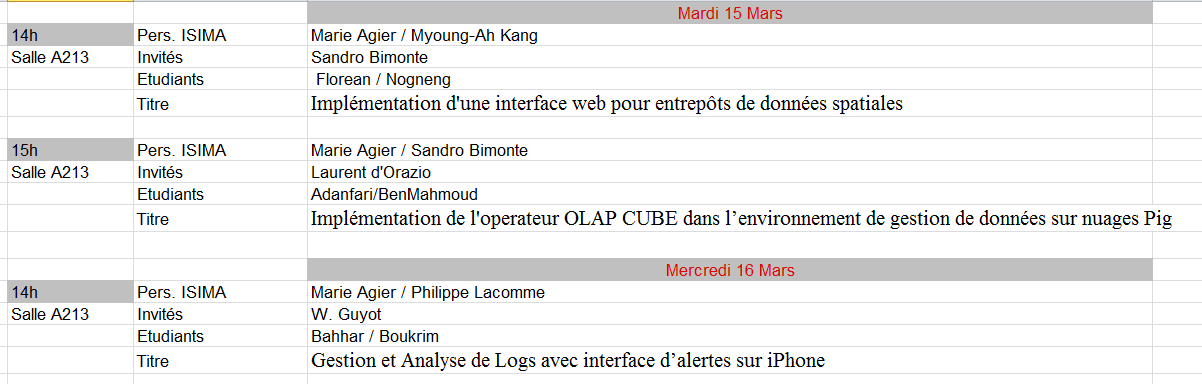
\includegraphics[scale = 0.45]{CalendrierSoutenance.png}
   \end{center}
  \caption{Exemple d'un planning de soutenances.}
\end{figure}
 
\subsection{Évaluation du projet}

\normalsize{
Après la soutenance, il est demandé aux tuteurs d'évaluer le travail des étudiants. Pour cela il existe un formulaire ( fourni en annexe) à remplir. Les critères d'évaluation ne sont pas seulement axés sur la qualité du travail accompli mais aussi le comportement (assiduité, communication etc). Les évaluations peuvent aller de très insuffisant à excellent. En plus, de l'évaluation du projet : il est demandé aux participants de la soutenance d'évaluer la performance de l'exposé réalisé part les étudiants.
}
\section{Critique de l'existant}

\normalsize{
Le processus de gestion de projet existant comporte certaines failles qui présentent un risque pour l'ISIMA.
}

\subsection{La proposition de projet}

\normalsize{
Le fait que la gestion des propositions de projet soient dépendantes des filières est problématique. En effet une proposition refusée par un responsable aurait pu intéresser une autre filière. De plus d'un point de vue de la communication, il est difficile pour l'ISIMA de refuser toutes les propositions de projet d'une entreprise au risque de rompre la collaboration avec l'école. Le fait que les responsables de fillières réceptionnent les propositions scinde la gestion de projet en deux, les premières années et les deuxièmes/troisièmes années.  
}

\subsection{Planification des soutenances}

\normalsize{
La planification faite par les responsable de filière à l'aide d'Excel peut poser des problèmes de coordination. En effet, le problème de versionning de ce type de fichier est récurrent ce qui engendre la mauvaise diffusion des modifications faites sur le calendrier d'où les quiproquos qui ont pu exister sur certaines dates de soutenance.
}

\subsection{Évaluation du projet}

\normalsize{
Les critères d'évaluation pour chaque filière sont différents ce qui peut provoquer une mauvaise uniformisation des résultats entre les filières. De plus, la soutenance n'étant pas officielle en première année, ce type de formulaire n'est pas utilisé pour l'évaluation, ce qui a pour effet de radicaliser les notes de projet de première année. 
}

\section{Idées d'amélioration}

\normalsize{
Ces propositions pourront servir de cas d'utilisation d'applications qui utiliseront la base de données qui va être créée pour la gestion de projet.
}

\subsection{La proposition de projet}

\normalsize{
Le fait d'avoir une base de données dédiée aux projets permettra de centraliser via une interface commune les propositions faites par les laboratoires et les entreprises. Ce qui résoudra les problèmes de pertes de propositions. De plus, il sera très facile de récupérer pour une entreprise ou laboratoire le ratio propositions acceptées / propositions refusées afin de maintenir avec eux des relations de collaborations convenables. Ces propositions ne pourront être visibles que par les responsables de filière avant validation. Les propositions validées seront visibles par les élèves de la filière concernée.     
}

\subsection{Planification des soutenances}

\normalsize{
La centralisation des données de planification des soutenances corrigera le problème de versionning des calendriers. Cette partie de la base de données pourra être associée aux logiciels de gestion des emplois du temps et des salles. 
}

\subsection{Évaluation du projet}

\normalsize{
Pour être consultables et stockables facilement les fiches d'évaluation doivent être uniformisées. Le modèle utilisé par la filière 2 et la filière 3 pourra être utilisé pour les autres filières ainsi que pour les premières années.  
}

%%%%%%%%%%%%%%%%%%%%%%%%%%%%%%%%%%%%%%%%%%%%%%%%%%%%%%%%%%%%%%%%%%%%%

\chapter {Modélisation de la base de données}

\section{Recensement des entités }

\normalsize{
Après analyse générale de la problématique de gestion de projets à l'ISIMA, j'ai pu identifier les identités suivantes :
}

\begin{itemize}
\item Entreprise.
\item Étudiant.
\item Évaluation.
\item Jury.
\item Keyword.
\item Outil.
\item Projet.
\item Proposition.
\item Responsable.
\item Soutenance. \\
\end{itemize}

\normalsize{
Chaque entité va être analysée afin d'en extraire les attributs et les liaisons qu'elle peut avoir avec d'autres entités.
}

\subsection{Entreprise}

\normalsize{
Entreprise est l'entité qui a proposé le sujet. Entreprise peut être aussi un laboratoire de recherche. On a besoin pour notre cas de l'adresse de l'entreprise. Cette table pourra être complétée par d'autres besoins issus des autres mini-projets. Par contre, cette table est liée à l'entité Responsable. Cette liaison permet de déterminer pour quelle entreprise travaille le responsable de projet.
}

\subsection{Étudiant}
\normalsize{
Comme pour l'entité entreprise. On a besoin que du nom et du prénom des élèves qui réalisent les projets. Elle pourra être complétée par d'autres besoins issus des autres mini-projets. Un étudiant peut être lié à un ou plusieurs projets.
}

\subsection{Évaluation}
\normalsize{
Cette entité se base sur les fiches d'évaluation de projet pour les filières F2 et F3. L'évaluation se décompose en deux parties. La première note le travail effectué sur le projet. La deuxième traite de la qualité de la soutenance. Chaque partie possède plusieurs critères avec des notes allant de très insuffisant à excellent. Cette évaluation est directement liée à un projet de façon unique.
}


\subsection{Jury}
\normalsize{
Le jury est composé des personnes qui assistent à la soutenance du projet. Pour les deuxièmes années, il s'agit de M.Mouzat ou de E.Hassinger qui évalue la partie communication et pour les troisièmes années il s'agit du responsable de filière. Pour le jury, il est nécessaire d'avoir son prénom et son nom ainsi que les éléments classiques de contacts (mail, téléphone). Un jury est lié à au moins une soutenance.
}

\subsection{Keyword}
\normalsize{
Cette entité provient de la présence de mots-clés dans les fiches de proposition de projet. En effet, il est intéressant de catégoriser les projets qui sont parvenus à l'ISIMA. D'une part pour faciliter le choix des étudiants et d'autre part pour permettre de faire des recherches par keyword dans l'historique. Les keyword décrivent les propositions de projet et les projets.
}


\subsection{Outil}
\normalsize{
Dans les fiches de propositions de projet il existe un champs outil. Cet élément me semble nécessaire dans la description générale du projet. Il permet de définir l'environnement de travail ce qui peut influer le choix des étudiants. Pour éviter la surcharge d'informations, chaque outil pourra être associé à une ou plusieurs filières. Par ex : Le serveur d'application jBoss sera adapté aux F2 et aux F3. Les outils sont reliés à au moins un projet.
}

\subsection{Projet}
\normalsize{
L'entité projet est l'entité principale de ce travail. Les attributs concernant les projets ont été récupérés sur les fiches de proposition de projet des F2 et des F3. L'entité comporte toutes les informations relatives au travail à fournir ainsi que les conditions de travail avec l'entreprise qui a proposé le projet.
}

\subsection{Proposition}
\normalsize{
L'entité proposition est identique à l'entité Projet. Son existence est due au fait qu'il est nécessaire de différencier une proposition d'un projet validé par un responsable de filière.
}

\subsection{Responsable}
\normalsize{
Les responsables sont les personnes qui supervisent les étudiants lors de leur réalisation de projet. Il est nécessaire de stocker leurs informations de contacts ( nom, prénom, adresse, mail et numéro de téléphone). Il peut y avoir plusieurs responsables pour un projet donné.
}

\subsection{Soutenance}
\normalsize{
L'entité soutenance permet de regrouper toutes les informations relatives à la planification de l'exposé des élèves (date et salle). La soutenance est reliée à un projet. 
}

\section{Schéma relationnel de la base de données}

\normalsize{
L'analyse des entités de la base de données permet d'extraire le schéma relationnel de la base de données. \\
}

\normalsize{
\noindent
PROJET ( \underline{idProjet}, sujet, filière, année, descriptif, environnement, travailExt, rémunération, convention, remarques)\\ \\
PROPOSITION ( \underline{idProposition}, sujet, filière, année, descriptif, environnement, travailExt, rémunération, convention, remarques)\\ \\
EVALUATION ( \underline{idEvaluation}, assiduité, progression, espritInitiative, communication, organisation, objectif, qualite, documentation, rapport, presentation, expression, question, noteProposee, noteReele, commentaires ) \\ \\
KEYWORD ( \underline{idKeyword}, intitule)\\ \\
OUTIL ( \underline{idOutil}, nomOutil, filiere)\\ \\
ETUDIANT ( \underline{idEtudiant}, nomEtudiant, prenomEtudiant)\\ \\
RESPONSABLE ( \underline{idResponsable}, nomResponsable, prenomResponsable, adresseResponsable, mailResponsable, telephoneResponsable)\\ \\
JURY ( \underline{idJury}, nomJury, prenomJury, mailJury, telephoneJury)\\ \\
ENTREPRISE ( \underline{idEntreprise}, adresseEntreprise)\\ \\
SOUTENANCE(\underline{\#idSoutenance}, dateSoutenance, salleSoutenance) \\ \\
PROPOSITIONOUTIL(\#idProposition, \#idOutil) \\ \\
PROJETOUTIL(\#idProjet, \#idOutil) \\ \\
PROPOSITIONKEYWORD(\#idProposition, \#idKeyword) \\ \\
PROJETKEYWORD(\#idProjet, \#idKeyword) \\ \\
PROJETEVALUATION(\#idProjet, \#idEvaluation) \\ \\
PROJETRESPONSABLE(\#idProjet, \#idResponsable) \\ \\
PROPOSITIONRESPONSABLE(\#idProposition, \#idResponsable) \\ \\
AFFECTATIONETUDIANT(\#idProjet, \#idEtudiant) \\ \\
AFFECTATIONJURY(\#idProjet, \#idJury) \\ \\
RESPONSABLEENTREPRISE(\#idEntreprise, \#idResponsable) \\ \\
}

\section{Schéma du modèle EA de la base de données}

\normalsize{
Ce schéma a été réalisé à l'aide du logiciel Dia.  
}

\begin{figure}[h]
   \begin{center}
   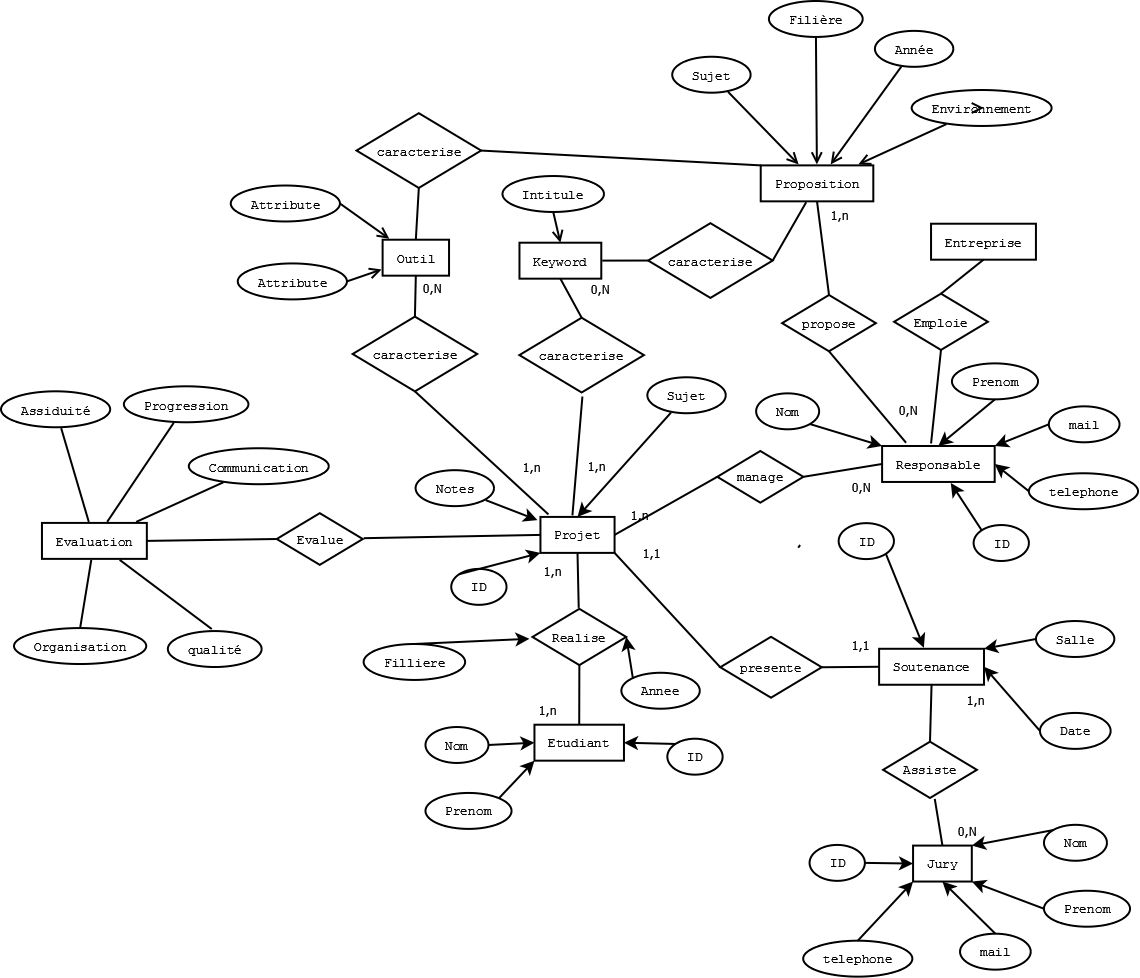
\includegraphics[scale = 0.29]{GestionProjet.png}
   \end{center}
  \caption{Schéma E/R de la modélisation de la base de gestion de projet.}
\end{figure}

%%%%%%%%%%%%%%%%%%%%%%%%%%%%%%%%%%%%%%%%%%%%%%%%%%%%%%%%%%%%%%%%%%%%%
\chapter {Utilisation de la base de données}

\section{La gestion de projets/soutenances}
\normalsize{
L'utilisation directe de la base de données serait une application web qui possèderait 3 interfaces :
}

\begin{itemize}
\item Étudiant.
\item Responsable ISIMA.
\item Propriétaire du projet.\\
\end{itemize}

\normalsize{ 
La première vue permettre aux étudiants de consulter les offres de projets qui leurs sont destinées et de valider leurs vœux. La deuxième vue réservée aux responsables de projets du côté de l'ISIMA permettra de voir en temps réel quels sont les projets qui ont été délaissé par les étudiants afin de pouvoir les répartir sur les autres filières ou sur les autres promotions de l'école. La troisième et dernière vue ajoutera une fonctionnalité de suivi de de la demande effectuée par une entreprise. Le demandeur pourra alors voir les étudiants qui ont été affectés au projet et ainsi faciliter la communication au sein du projet. Ce type d'application permettrait de professionnaliser la gestion de projets et concorderai avec la démarche qualité qui est en cours au sein de l'ISIMA.
}

\section{Cooccurrence des données}
{
L'une remarques qui a été souvent remontés au niveau des alternants est la redondance de certaines données entre les différents modèles proposés. En effets, les informations sur les entreprises ou les étudiants ont été souvent nécessaires dans les études de cas. Pour des raisons évidentes, il est nécessaire de centraliser ce type d'informations. C'est pour cela qu'on pourrait imaginer un portail applicatif qui rassemblerait les études faites par mes camarades. De plus certaines fonctionnalités pourraient collaborer parfaitement (Ex : Le forum ISIMA avec la gestion des stages et des projets pour remplir automatiquement les champs concernant l'expérience professionnelle). Certes, un développement personnalisé ne serait pas envisageable dans un cas comme l'ISIMA mais ce type d'approche pourrait être approfondi avec des interactions avec le progiciel Apogée.
}

\chapter{Entrepôt de données}

\section {Introduction aux entrepôts de données}

\normalsize{
L'objectif à atteindre est complètement  différent des bases de données "traditionnelle". En effet, tandis que les bases de données relationnelles cherchent à stocker le plus proprement possible les données d'une entreprise ou d'une application, les entrepôts ont pour but de fournir un grand nombre d'informations décisionnelles aux dirigeants de l'entité. Ces informations serviront aux prises de décisions stratégique de l'entité. L'objectif à atteindre n'est pas la seule différence avec les bases de données traditionnelles. Elles ont une architecture très opposées l'une à l'autre. Les bases relationnelles éclatent au maximum leur schéma afin d'éviter la redondance au détriment de la performance. Pour les bases décisionnelles , la redondance des informations n'est pas un critère de construction. Les schéma des entrepôts de données se décomposent en deux parties : les faits et les dimensions. Voici un exemple d'architecture en étoile pour un entrepôt.
} 

\begin{figure}[h]
   \begin{center}
   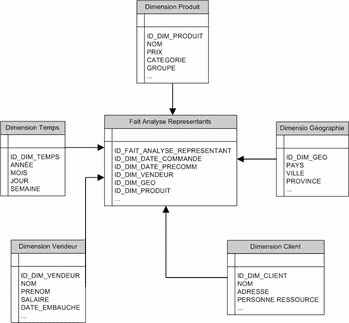
\includegraphics[scale =1.0]{etoile.png}
   \end{center}
  \caption{Schéma en étoile.}
\end{figure}

\normalsize{
Le but final de l'entrepôt de données pour un décideur serait d'obtenir une z = f(x,y,z,...) où x,y,z, serait des valeurs des dimensions et où z serait un élément provenant ou calculé à partir de la table des faits. 
}

\section{Application de l'entrepôt de données à l'ISIMA}

\normalsize{
Actuellement, il existe aucun élément des systèmes d'informations qui permette de réaliser des statistiques concernant la vie étudiante. En effet, il serait intéressant pour l'école, par exemple, de connaître le nombre d'élèves par type de recrutement (BTS, Prépas, IUT, etc) et de voir quel est le type de formation qui réussit le mieux à l'ISIMA. Pour compenser ce manque, mes camarades et moi avons modélisé une structure qui pourrait convenir pour un entrepôt de données pour l'ISIMA.\\ Voici les dimensions qui ont été retenues :
}
\begin{itemize}
\item Entreprise.
\item Les informations concernant le BAC de l'élève.
\item Le niveau de l'étudiant (année, filière).
\item La nationalité.
\item Le provenance académique de l'étudiant (IUT,Prépa,BTS etc...).\\
\end{itemize}

\normalsize{
Pour la table de fait on obtient :
}

\begin{itemize}
\item Sexe.
\item LV2,LV3.
\item Age.
\item Redoublant.
\item Mention Bac.
\item Catégorie socio-professionnelle des parents.\\
\end{itemize}

\normalsize{
Le script de création de la table complète est disponible en annexe. 
}

\section{Exploitation de l'entrepôt de données}

\normalsize{
Les entrepôts de données peuvent être exploités de plusieurs manières, mais la plus cohérente avec notre utilisation de la méthodologie OLAP.
}

\begin{figure}[h]
   \begin{center}
   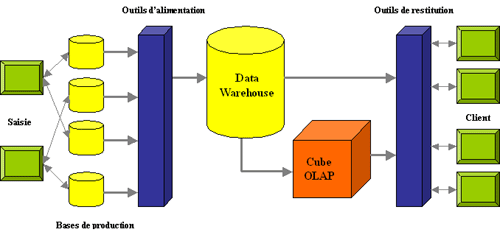
\includegraphics[scale =1.0]{architecture_general.png}
   \end{center}
  \caption{Architecture générale des entrepôts de données.}
\end{figure}

\vspace{0.5cm}
\normalsize{
Voici une définition de la méthodologie OLAP trouvé sur le site de l'université de d'Annecy. \\
}

\begin{quote}
Un cube OLAP est une représentation abstraite d'informations multidimensionnelles exclusivement numérique utilisé par l'approche OLAP (acronyme de On-line Analytical Processing). Cette structure est prévue à des fins d'analyses interactives par une ou plusieurs personnes (souvent ni informaticiens ni statisticiens) du métier que ces données sont censées représenter. 

Les cubes OLAP ont les caractéristiques suivantes : \\

1- obtenir des informations déjà agrégées selon les besoins de l’utilisateur.\\
2- simplicité et rapidité d’accès\\
3- capacité à manipuler les données agrégées selon différentes dimensions\\
4- un cube utilise les fonctions classiques d’agrégation : min, max, count, sum, avg, mais peut utiliser des fonctions d’agrégations spécifiques.\\ \\
\end{quote}

\normalsize{
\noindent
Voici, un exemple de résultat graphique que l'on peut obtenir avec les données de l'ISIMA.
}

\begin{figure}[h]
   \begin{center}
   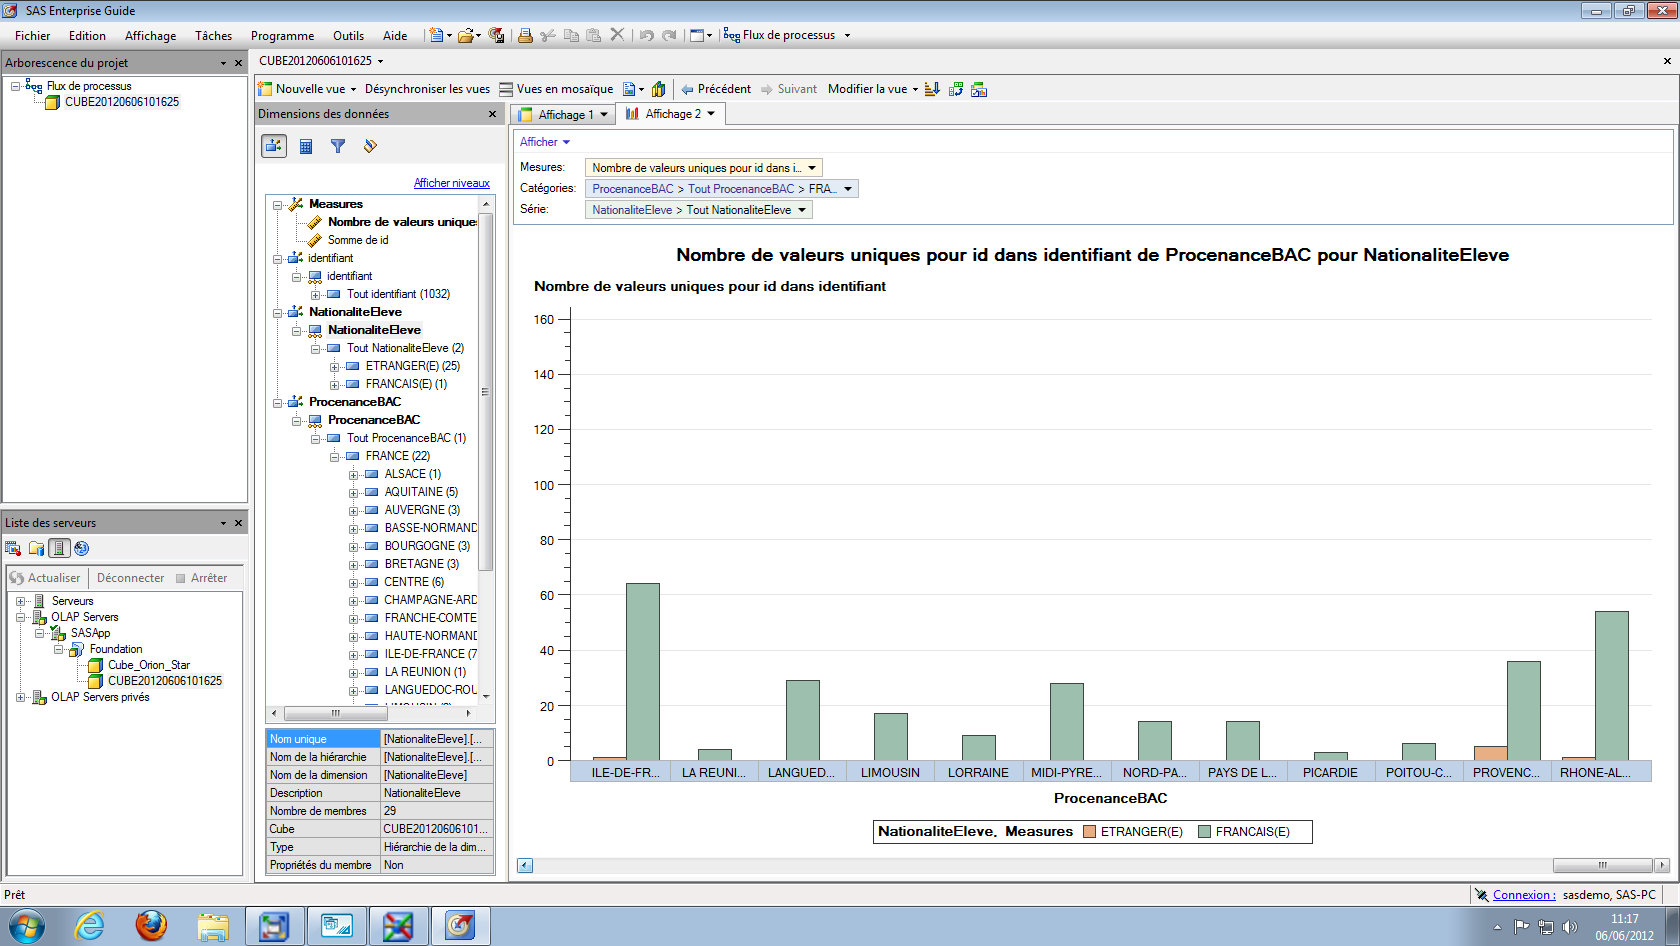
\includegraphics[scale =0.35]{resultatNatCube.png}
   \end{center}
  \caption{Nombre d'élèves par région de bac.}
\end{figure}

\chapter{Conclusion}

\normalsize{
Le but de ce cours était de prendre conscience des enjeux stratégiques que peuvent avoir les systèmes de données et comment l'application de méthodes de structuration peut simplifier le travail des gens. De plus, cette prise de recul m'a permis de concevoir les systèmes d'informations avec plus de hauteur qu'à l'accoutumée avec mon point de vue plus développeur.
Ce rapport ne traite pas de la partie "Data Quality" même si cela a été un point-clé de l'étude. En effet, la plus grosse difficulté a été de trouver le bon format pour les données à traiter. Et comme j'ai pu le constater avec les fichiers d'entrée que j'ai obtenue lors de mon étude sur la gestion de projets à l'ISIMA. La plus grosse partie du travail est la collecte et l'uniformisation des données. Dans le cas de l'ISIMA, la question de repartir de zéro peut se poser tant les données sont hétérogène.
}

\normalsize{
D'un point de vue strictement personnel, l'utilisation d'outil ETL comme Talend ne m'a pas été marquante. Par contre, le fait qu'un système de donnée bien organisé peut complètement modifier l'efficacité d'une entité et m'a fait prendre conscience qu'il faut absolument donner aux utilisateurs les moyens de communiquer et collaborer ensemble au travers d'applications communes. 
}

\end{document}